\documentclass{report}

\usepackage{fullpage}
\usepackage{url}
\usepackage{amsthm}
\usepackage{amsmath}
\usepackage{amssymb}
\usepackage{cite}
\usepackage{listings}
\usepackage{graphicx}

\usepackage{tkz-graph}
\usetikzlibrary{arrows}
\usetikzlibrary{shapes}

\theoremstyle{plain}
\newtheorem{theorem}{Theorem}
\newtheorem{proposition}{Proposition}
\newtheorem{lemma}{Lemma}
\newtheorem*{corollary}{Corollary}

\theoremstyle{definition}
\newtheorem{definition}{Definition}
\newtheorem{conjecture}{Conjecture}
\newtheorem{example}{Example}
\newtheorem{algorithm}{Algorithm}

\theoremstyle{remark}
\newtheorem*{remark}{Remark}
\newtheorem*{note}{Note}
\newtheorem{case}{Case}

\numberwithin{definition}{chapter}
\numberwithin{example}{chapter}
\numberwithin{figure}{chapter}
\numberwithin{theorem}{chapter}
\numberwithin{lemma}{chapter}

\SetVertexNormal[Shape      = circle,
                 FillColor  = blue!20,
                 LineWidth  = 2pt]
\SetUpEdge[lw         = 2pt,
           color      = black,
           labelcolor = white,
           labeltext  = red,
           labelstyle = {sloped,draw,text=blue}]

\title{Parallelising graph algorithms in HPC-GAP \\ \vspace{2 mm} {\large University of St Andrews}}
\author{Ivars Zubkans \\ \small Supervised by: Dr James D Mitchell}

\begin{document}

\maketitle

\begin{abstract}

The GAP system for computational discrete algebra did not have a general purpose package for general graphs and graph theoretic algorithms. Moreover, parallelism capabilities were recently added in a high performance version of GAP. Therefore, this project implements a general purpose package for working with graphs. In addition, it is explored how the implemented algorithms can be modified to suit parallel execution. If efficient parallelism modifications were not found, different algorithms better suited for parallel execution were introduced. This paper describes in detail how one can find strongly connected components of a graph using the Gabow's algorithm for serial execution and how they can be found using the forwards-backwards algorithm for parallel execution. Moreover, possible optimizations of the forwards-backwards algorithm are described. Furthermore, ways of how to find only the required strongly connected components without wasting computation are found. In addition, this paper describes in detail exact algorithms for vertex coloring, namely brute force and backtracking algorithms. The backtracking algorithm was optimized by reordering vertices and modifications for parallel execution of both algorithm were made.

\end{abstract}

TODO declaration.

\tableofcontents

\chapter{Introduction}

Efficient implementations of graph theoretic algorithms are important due to their heavy use for modelling and solving problems in various fields. A graph represents connections between a set of objects. These connections induce questions like are these two objects connected? Can we get from one object to another? How many objects can be reached from some specific object? What is the best way to reach another object and so on.

Thus graphs can be used to model relations in information, physical and social systems \cite{6005872}. Graph theory is used in areas of computer science such as data mining, image segmentation, clustering, image capturing and networking \cite{6005872}. Problems of efficiently planning network routes and diagnosing faults in computer networks are solved using graphs \cite{6005872}. In chemistry and physics graphs are used to study molecules, atoms and construction of bonds \cite{shirinivas2010applications}. In biology graphs are used to model inhabitance regions of certain species and their migration paths \cite{shirinivas2010applications}. Similarly, graph theory is used in sociology to measure actors prestige or to explore diffusion mechanisms \cite{shirinivas2010applications}.

The aim of the project was to explore and implement serial and parallel versions of graph algorithms in GAP. The GAP (\url{www.gap-system.org}) is a free open-source program for computing with various mathematical structures such as graphs, groups and fields. The graph related algorithms are in a package called Graph Algorithms Using Permutation Groups (GRAPE). This package is primarily used for working with graphs related to groups, finite geometries and designs. Thus it focuses on highly symmetric graphs to take advantage of the symmetries. There is no package for more standard graph algorithms such as traversal, path finding, minimum spanning tree algorithms and strongly connected components.

Moreover, in a recent addition, HPC-GAP supports parallelism with both shared and distributed memory models. A shared memory can be used simultaneously by multiple programs to provide communication and remove redundancy \cite{berman1996fundamentals}. In a distributed memory each central unit of processing (CPU) has its own private memory \cite{berman1996fundamentals}. Furthermore, all of the current implementations in GRAPE are non-parallel, while we would like to take advantage of the parallelism capabilities to execute our programs faster. The project's motivation is solving both of these problems --- the lack of a general graphs package and not taking advantage of the parallelism capabilities. Therefore this project aimed to create packages for working with graphs and solving some classical graph algorithm problems both for serial and parallel execution.

During the project two GAP packages were made one for serial and another for parallel implementations. Each made package is a self-contained extension to the core system of GAP. The serial package contains implementations for doing breadth first search, depth first search and solving vertex colouring, strongly connected components, minimum spanning trees and Dijkstra's shortest paths problems. These problems were picked, because they are some of the most common graph problems with many applications and are usually found in texts on graph theoretic algorithms.

In this submission we will describe in detail the implementations of the strongly connected components and vertex colouring algorithms, while briefly explaining breadth first and depth first search. For both covered algorithms we define the problems themselves, give examples of their applications and look at how we can solve them. The target audience of this text a subhonours student with some background of pure mathematics and very brief knowledge of programming. The reader should be comfortable with working with abstract definitions, theorems and proofs and reading simple pseudo code.

The packages source code can be found at a mercurial repository
\url{http://mercurial.selenic.com/} on bitbucket \url{https://bitbucket.org/}. The url of the repository is \url{https://bitbucket.org/IvarsZ/parallelgraphs}. It can be accessed through a web browser or cloned for local browsing and execution. In the "pkg/graphs" and "pkg/pgraphs" folders there are a README files that desribe how to generate documentation for the packages. In the "doc" folder there is a tex file "Report.tex" that describes another separate part of the project including specific implementation details -- how packages are structured and graphs represented in detail, the other algorithm implementations and how random graphs can be generated for experiments.

Now we will introduce the basic definitions and lay a foundation for the next chapters.

\section{Basic Graph Definitions}

A graph represents connections or relationships, called edges, between a set of elements, called vertices, more formally.

\begin{definition}[Graph]
A $graph$  $G$ is an ordered triple $G = (V, E, ends)$ where $V$ and $E$ are sets, while $ends$ is a function 
  \begin{equation}
  ends:E\to \mathcal P \left({V}\right)
  \end{equation}
which assigns to each element of $E$ a set of one or two elements of $V$. The elements of $V$ are called $vertices$ or $nodes$ of $G$, and elements of $E$ are called $edges$ of $G$ \cite{bondy2008graph}.
\end{definition}

The above definition is the one that will be used throughout the text instead of the most common graph definition:

\begin{definition}[Graph]
A $graph$  $G$ is an ordered pair of disjoint sets $G = (V, E)$ where $E$ is a subset of the set $V^{(2)}$ of unordered pairs of V, not necessarily distinct \cite{bollobas1998modern}. 
\end{definition} 

In the second definition the edges between vertices are defined implicitly in terms of vertices and it is less clear that edges are separate objects that define the relationships between vertices. Therefore the first definition is used. Furthermore, the first definition includes the second, but the second definition does not include the first. The second definition does not allow multiple edges between the same pair of vertices since in a set of edges there can be only one subset of the pair of vertices.

We will consider only $finite \ graphs$ - graphs with finite number of vertices and edges, because the algorithmic problems and their considered solutions work in finite time only on finite graphs.

\begin{example}
An example of a graph is $G=(V, E, ends)$ where $V=\{1,2,3,4,5\}$, $E=\{\{1,2\}, \{2,3\}, \{3,1\}$, $\{4,3\}\}$ and is defined by the identity map, since $E \subseteq P(V)$. This illustrates how both graphs defined using the second definition could be defined using the first definition.

\begin{figure}[h]
\center
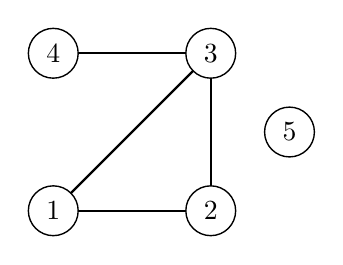
\begin{tikzpicture}
   \Vertex[x=0 ,y=0]{1}
   \Vertex[x=2,y=0]{2}
   \Vertex[x=2 ,y=2]{3}
   \Vertex[x=0 ,y=2]{4}
   \Vertex[x=3 ,y=1]{5}
   \Edge(1)(2)
   \Edge(2)(3)
   \Edge(3)(1)
   \Edge(3)(4)
\end{tikzpicture}
\caption{Graphical representation of a (simple, undirected) graph.}
\end{figure}
\end{example}

\begin{definition}[Incident]
Let $G = (V, E, ends)$ be a graph and $v\in V$ be a vertex, then $v$ is $incident$ to an edge $e \in E$ if $v \in ends(e)$.
\end{definition}

\begin{definition}[Adjacent]
Let $G = (V, E, ends)$ be a graph and $v,w\in V$ be vertices, then $v$ and $w$ are adjacent if there is an edge $ e \in E$ such that $ends(e) = \{v, w\}$.
\end{definition}

\begin{definition}[Loop]
Let $G = (V, E, ends)$ be a graph and $e \in E$ be an edge , then $e$ is a $loop$ if $ends(e) = \{v\}$ for some vertex $v \in V$.
\end{definition}

\begin{definition}[Simple graph]
Let $G = (V, E, ends)$ be a graph, then $G$ is simple if
\begin{itemize}
\item $V$ is finite,
\item $G$ has no loops,
\item for any pair of vertices $v,w \in V$ there is at most one edge $e \in E$ such that $ends(e) = \{v, w\}$, i.e. there is at most one edge connecting a pair of vertices.
\end{itemize}
\end{definition}

We will generally consider simple graphs, but all of the implemented algorithms work on graphs with multiple edges between two vertices or on graphs with loops. Of course they do not work for infinite graphs. We consider simple graphs, because they are easier to work with.

\begin{example}
The graph in the next example (figure \ref{loop}) has a loop at 4, so it is not simple. And for example the vertices 1 and 2 are adjacent, while 1 and 4 are not. Moreover, the edge between the vertices 1 and 2 is incident to 1 and 2.
\begin{figure}[h]
\center
\begin{tikzpicture}
   \Vertex[x=0 ,y=0]{1}
   \Vertex[x=2,y=0]{2}
   \Vertex[x=2 ,y=2]{3}
   \Vertex[x=0 ,y=2]{4}
   \Vertex[x=3 ,y=1]{5}
   \Edge(1)(2)
   \Edge(2)(3)
   \Edge(3)(1)
   \Edge(3)(4)
   \Loop[style={}](4)
\end{tikzpicture}
\caption{An example of graph with a loop}
\label{loop}
\end{figure}
\end{example}

\begin{definition}[Path]
Let $G = (V, E, ends)$ be a graph, then a $path$ in $G$ is a sequence, $P$, of vertices $v_1,v_2,..,v_n$ such that $v_i$ and $v_{i+1}$ are adjacent for $1 \leq i \leq n - 1$, we say that $P$ is a path between $v_1$ and $v_n$.
\end{definition}

\begin{definition}[Connected]
Let $G = (V, E, ends)$ be a graph, then $G$ is $connected$ if there exists a path between any pair of vertices in $V$ \cite{bollobas1998modern}.
\end{definition}

\begin{definition}[Subgraph]
Let $G = (V, E, ends)$ be a graph, then a subgraph of $G$ is a graph $G'=(V', E', ends')$ such that $V' \subseteq V$, $E' \subseteq E$ and $ends'$ is a restriction of $ends$ to $E'$ \cite{bondy2008graph}.
\end{definition}

\begin{definition}[Connected Component]
Let $G = (V, E, ends)$ be a graph, then a maximal connected subgraph of $G$ is called a $connected \ component$ \cite{bollobas1998modern}.
\end{definition}

Checking connectedness and finding connected components of a (undirected) graph is relatively easy, because if there is a path from a vertex $v$ to a vertex $w$, then there is a path from $w$ to $v$, i.e. connectedness is symmetric in (undirected) graphs. The connected components can be found by using breadth first search (BFS) or depth first search (DFS). Just pick a vertex and find all of its connected vertices using BFS or DFS. Repeat the process for vertices not yet in any component.

BFS visits vertices level by level - the vertices closer to the starting vertex are visited first. For that it uses a First-In-First-Out (FIFO) queue, where all adjacent undiscovered vertices of the vertex being visited are enqueued and marked as discovered \cite{c++_sedgewick}. Meanwhile DFS visits a path as far as it can before backtracking until the latest branching option in the path options considered. It uses a Last-In-First-Out (LIFO) stack, where all adjacent undiscovered vertices of the vertex being visited are pushed on the stack and marked as discovered \cite{c++_sedgewick}. So both BFS and DFS are very similar, except that the order in which they visit vertices is different. Since BFS and DFS consider each edge and vertex only once they have linear time complexity - $O(|V| + |E|)$. For more detail on BFS and DFS, queues and stacks, and how they were implemented see the attached computer science submission.

\section{Basic Algorithm Definitions}

\begin{definition}[Algorithm]
An $algorithm$ is a complete, step-by-step procedure for solving a specific problem in a finite amount of time. Each step has to be unambiguous and expressed in terms of finite number of rules \cite{berman1996fundamentals}.
\end{definition}

The rise of multi-processor and multi-core architectures has made the distinction between serial (sequential) and parallel algorithms an important one.

\begin{definition}[Serial Algorithm]
A $serial \ algorithm$ performs its steps in a sequence one at a time \cite{berman1996fundamentals}.
\end{definition}

\begin{definition}[Parallel Algorithm]
A $parallel \ algorithm$ performs many of its steps at the same time \cite{berman1996fundamentals}.
\end{definition}

We would like to compare different algorithms and analyse their theoretical performance without implementing them. Therefore we need to abstract away machine dependant details. The most common way of doing this is to use a hypothetical computer called $the Random Access Machine$. In Random Access machine every simple operation takes (arithmetic operations, branching, function calls) takes exactly one time step and loops are compositions of the simple operations. Furthermore, memory access takes exactly one time step, as caching is ignored and we assume we have enough random access memory \cite{skiena504algorithm}. Of course not all operations take exactly the same time, but this model is simple and captures the behaviour of a computer well enough. Therefore it is used despite its limitations.

This model allows us to count the number of steps an algorithm will take on a specific instance of a problem, so it only tells how good or bad and an algorithm is on a specific instance. Therefore we define worst-case, best-case and average-case complexities.

\begin{definition}[Worst-case complexity]
The \emph{worst-case complexity} of an algorithm is a function on natural numbers --- the maximum number of steps taken by the algorithm on any instance of size $n$ \cite{skiena504algorithm}.
\end{definition}

\begin{definition}[Average-case complexity]
The \emph{average-case complexity} of an algorithm is a function on natural numbers --- the average number of steps taken by the algorithm on any instance of size $n$ \cite{skiena504algorithm}.
\end{definition}

\begin{definition}[Best-case complexity]
The \emph{best-case complexity} of an algorithm is a function on natural numbers --- the minimum number of steps taken by the algorithm on any instance of size $n$ \cite{skiena504algorithm}.
\end{definition}

Best-case complexity is fairly useless in practice, because an algorithm could be really good on one instance (e.g. with a hard-coded solution), and really bad and take a very long time on all other instances. Average-case complexity is hard to use, because determining and characterising mathematically average inputs is difficult. Therefore we will generally use worst-case complexity.

Unfortunately these functions are often very complicated, therefore we will use their upper and lower bounds and discard their growth rates, because we mostly care about how the algorithms scale anyway.

\begin{definition}[Upper bound]
A function $g(n)$ is an $upper \ bound$ of a function $f(n)$ if there exists some constant $c$ such that $f(n)\leq cg(n)$ always holds for large enough $n$. It is denoted by $f(n) = O(g(n))$ \cite{skiena504algorithm}.
\end{definition}

\begin{definition}[Lower bound]
A function $g(n)$ is an $lower \ bound$ of a function $f(n)$ if there exists some constant $c$ such that $f(n)\geq cg(n)$ always holds for large enough $n$. It is denoted by $f(n) = \Omega(g(n))$ \cite{skiena504algorithm}.
\end{definition}

\begin{definition}[Exact bound]
A function $g(n)$ is an $exact \ bound$ if it is both a lower and an upper bound (with possibly different constants) on another function $f(n)$, then it is denoted by $f(n) = \Theta(g(n))$
\end{definition}

We will generally try to find an upper bound, because the exact bound is usually harder to find and the lower bound is generally useless on its own. Note, this ignores the constant growth factor of the complexity, i.e. functions $5n^2$ and $2n^2+1$ have the same lowest upper bound of $n^2$, therefore sometimes in practice one has to consider the growth factor at least for functions with the same lowest upper bound.

An algorithm is considered efficient time wise if its time complexity is $O(n)=log(n)$, because the logarithm function grows very slowly. Note that the logarithm base does not really matter, as it does not have a big impact on scaling, although even polynomial time algorithms are considered good, especially when the polynomial is small. For parallel algorithms we strive to have a polylogarithmic worst-case complexity with a polynomial number of processors. Problems solvable by such algorithms are considered to be in the class called NC \cite{berman1996fundamentals}.

In this project we strived to implement algorithms that are correct and efficient, both time and memory wise, while being easy to implement. Unfortunately all three goals are not always achievable. Of course we placed the most emphasis on correctness, otherwise the implementations are useless. Therefore proofs of correctness are given. Note, heuristics, algorithms giving approximate answers, are not considered in this project, since we are interested in precise and exact answers. Next we consider the efficiency the most important, because it allows us to work with larger datasets faster without upgrading hardware. Despite that, a balance is struck between efficiency and ease of implementation, as implementing very complicated algorithms is beyond the scope of this project. Efficiency wise bigger emphasis was placed on time complexity than space complexity, since machines with many processors generally have a lot of available memory.

Parallel algorithms have issues and constraints only specific to them \cite{berman1996fundamentals}:

\begin{itemize}
  \item Single instruction versus multiple instruction architecture: in a single instruction architecture only the same instruction can be executed in parallel, but possibly on different data. While multiple instruction architecture does not have such a limitation. GAP follows multiple instruction architecture.
  \item Number and type of processors available: parallel architectures have varying number of processors of varying capabilities. In GAP it is assumed that all processors are powerful enough to execute all normal instructions of a serial machine.
  \item Shared versus distributed memory model: GAP supports both, but we will use the shared memory model as it is easier to work with.
  \item Read and write restrictions: in GAP standard techniques of read and write locks and atomic objects are used to control concurrent access to the shared memory.
\end{itemize}

Thus designing and implementing parallel algorithms is generally harder, therefore a number of approaches are used when designing parallel algorithms \cite{berman1996fundamentals}:
\begin{itemize}
  \item Modify an existing sequential algorithm exploiting those parts of the algorithm that are easily paralllizable. This approach is used to tackle vertex colouring.
  \item Come up with a completely new approach that does not have a natural sequential algorithm analogue or generally is not used for serial implementations. This often involves splitting the problem in smaller independent subproblems. Naive algorithms are sometimes better suited for parallelism as they have more redundancy and are not squeezing everything out of the problem. This approach is used for finding the strongly connected components.
  \item For some problems just execute the same algorithm with different starting conditions on many processors until one finds a solution or the whole search space is covered.
\end{itemize}

\section{Implemented Algorithms}
\begin{itemize}
  \item Breadth first search
  \item Depth first search
  \item Strongly connected components
  \item Vertex colouring
  \item Minimum spanning trees
  \item Single source shortest paths
\end{itemize}

These algorithms were picked, because they are some of the most common graph algorithms that solve the most common graph problems. The other popular graph problems are travelling salesman problem, graph isomorphism and clique problem. Furthermore, they cover a wide range of different graphs (directed, undirected, weighted) and a range of different time complexities from linear to exponential. Note, in this paper we describe only the strongly connected components, vertex colouring and single source shortest paths. For reference to other algorithms implemented see the computer science parts paper that is attached.

The graphs in both packages are represented using adjacency lists, i.e. the graph is a list of lists storing the adjacent vertices for each vertex of the graph. This approach was picked over adjacency matrix representation. For graphs with weights there is an additional list of lists storing the weights of edges. For more details on how the graphs are represented in the implementations and why, again see the computer science parts paper that is attached.

\chapter{Strongly Connected Components}

\section{Defining strongly connected components}

As discussed, edges in a graph represent relationships between vertices. Often these are not symmetric and are represented using directed graphs, where edges have direction, i.e. there is a start and end vertex for each vertex. In this chapter we will consider directed graphs and by a graph we will mean a directed graph, unless specified otherwise unlike in other chapters were by default a graph is undirected.

\begin{definition}[Directed graph]
A \emph{directed graph}, $G$, is a triple $G = (V, E, ends)$ where $V$ and $E$ are sets, while $ends$ is a function 
  \begin{equation}
  ends:E\to V \times V
  \end{equation}
which assigns to each element of $E$ a pair of two (possibly equal) elements of $V$ .
\end{definition}

\begin{definition}[Incident From]
Let $G = (V, E, ends)$ be a directed graph and $v \in V$ be a vertex, then $v$ is $incident \ From$ an edge $e \in E$ if $ends(e)=(v, w)$ for some vertex $w$.
\end{definition}

\begin{definition}[Incident To]
Let $G = (V, E, ends)$ be a directed graph and $v \in V$ be a vertex, then v is $incident \ to$ an edge $e \in E$ if $ends(e)=(w, v)$ for some vertex $w$.
\end{definition}

\begin{definition}[Adjacent To]
Let $G = (V, E, ends)$ be a directed graph and $v,w\in V$ be vertices, then $v$ is $adjacent \ to$ $w$ if there is an edge $ e \in E$ such that $ends(e) = \{v, w\}$.
\end{definition}

\begin{example}
An example of a directed graph is $G=(V, E, ends)$ where $V=\{1,2,3,4,5\}$, $E=\{(1,2), (2,3), (3,1)$, $(4,3)\}$ and is defined by the identity map, since $E \subseteq V^2$. Moreover, 1 is adjacent to 2, edge (1,2) is incident from 1 and incident to 2.

\begin{figure}[h]
\center
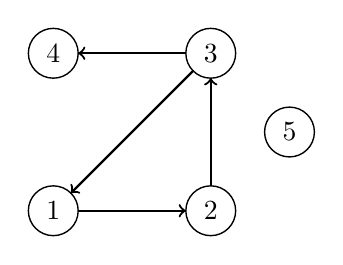
\begin{tikzpicture}
   \Vertex[x=0 ,y=0]{1}
   \Vertex[x=2,y=0]{2}
   \Vertex[x=2 ,y=2]{3}
   \Vertex[x=0 ,y=2]{4}
   \Vertex[x=3 ,y=1]{5}
   \tikzset{EdgeStyle/.style={->}}
   \Edge(1)(2)
   \Edge(2)(3)
   \Edge(3)(1)
   \Edge(3)(4)
\end{tikzpicture}
\caption{Graphical representation of a (simple) directed graph.}
\end{figure}
\end{example}

Now while checking connectedness and finding connected components is relatively easy in undirected graphs, It gets a bit more complicated for directed graphs, because there is not structural symmetry any more for categorizing connectedness. First, we need to distinguish between two different types of connectedness in directed graphs, because there are two directions for paths now --- "forwards" and "backwards".

\begin{definition}[Strongly Connected]
Let $G = (V, E, ends)$ be a directed graph, then two vertices $v, w \in V$ of $G$ are $strongly \ connected$ if there exists a path from $v$ to $w$ and there exists a path from $w$ to $v$.
\end{definition}

\begin{definition}[Weakly Connected]
Let $G = (V, E, ends)$ be a directed graph, then two vertices $v, w \in V$ of $G$ are $weakly \ connected$ if either there exists a path from $v$ to $w$ or there exists a path from $w$ to $v$.
\end{definition}

Now we can define strongly connected components.

\begin{definition}[Strongly Connected Component]
Let $G = (V, E, ends)$ be a graph, then a maximal strongly connected subgraph of $G$ is called a $strongly \ connected \ component$ of $G$.
\end{definition}

\begin{example}
Below is an example of strongly connected components of a directed graph. The components are subgraphs induced by vertices $\{1,6,3,4\}$, $\{2,7,8\}$, $\{5\}$ and $\{9\}$.

\begin{figure}[h]
\center
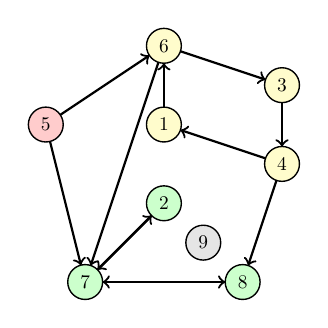
\begin{tikzpicture}[scale=0.5]
   \tikzset{EdgeStyle/.style={->}}
   \tikzset{VertexStyle/.append  style={fill=yellow!20, scale=0.7]}}
   \Vertex[x=0 ,y=0]{1}
   \tikzset{VertexStyle/.append  style={fill=yellow!20}}
   \Vertex[x=3,y=1]{3}
   \Vertex[x=3 ,y=-1]{4}
   \Vertex[x=0 ,y=2]{6}
   \tikzset{VertexStyle/.append  style={fill=green!20}}
   \Vertex[x=0 ,y=-2]{2}
   \Vertex[x=-2 ,y=-4]{7}
   \Vertex[x=2 ,y=-4]{8}
   \tikzset{VertexStyle/.append  style={fill=red!20}}
   \Vertex[x=-3 ,y=0]{5}
   \tikzset{VertexStyle/.append  style={fill=gray!20}}
   \Vertex[x=1 ,y=-3]{9}
   \Edge(6)(3)
   \Edge(3)(4)
   \Edge(4)(1)
   \Edge(1)(6)
   \Edge(4)(8)
   \Edge(6)(7)
   \Edge(2)(7)
   \Edge(7)(2)
   \Edge(7)(8)
   \Edge(8)(7)
   \Edge(5)(6)
   \Edge(5)(7)
\end{tikzpicture}
\caption{Strongly connected components of a directed graph}
\end{figure}
\label{SCC_example}
\end{example}

Now that we have defined strongly connected components, the goal of a strongly connected components algorithm is to partition the vertices $V$ of a directed graph $G=(V,E,ends)$ into strongly connected components. It is usually done by assigning component index numbers to each vertex, either starting from zero or $|V|$ (1 or $|V|+1$ for 1-index based programming languages), this also allows to easily determine the number of strongly connected components.

Finding strongly connected components allows to treat all vertices of a strongly connected component as the same, since they are reachable from each other. Strong connectedness is an equivalence relation and thus by finding equivalence classes of it in a graph we can remove redundancy from a graph by collapsing all strongly connected vertices to a single vertex to get an acyclic graph of strongly connected components. This allows to tell how well connected a network is. In addition strongly connected components can be used to solve 2-satisfiability problems \cite{aspvall1979linear}, in set oriented methods for the numerical study of discrete dynamical systems \cite{dellnitz2002set} and in the discrete ordinates method for modeling radiation transport \cite{fleischer2000identifying}.

\section{Serial algorithms}

The simplest approach to find strongly connected components is the brute force algorithm. Using DFS or BFS check for every pair of two vertices $v$ and $w$ that there is a path from $v$ to $w$ and from $w$ to $v$, i.e. just run BFS or DFS on $v$ and then on $w$ until $w$ and $v$ are found, respectively. Of course this algorithm is very inefficient. Its time complexity is $O(V^2E)$ (for a strongly connected graph). It is because we are repeating almost the same search for every pair of vertices in the same strongly connected component. Therefore we can do much better. As we will see later, strongly connected components can be found in linear time, i.e. its time complexity is $O(V + E)$.

The three most common algorithms for finding strongly connected components are Kosaraju's, Tarjan's and Gabow's algorithms. Moreover all three have linear time and space complexity \cite{c++_sedgewick}. Kosaraju's algorithm works by running DFS with postordering on the reverse (direction of edges is reversed) of the graph and then running a second DFS. After an iteration of the second DFS is exhausted. another one is started at a yet unvisited vertex with the highest postorder number given by the first DFS \cite{c++_sedgewick}. The Tarjan's algorithm is based on DFS and uses a stack to keep track of the current search path. A sequence of vertices is only popped from the top of the stack when it is determined that all of them are in the same strongly connected component. This happens when the last vertex of the strongly connected component is visited and can be determined by maintaining the lowest index  reachable vertex for each vertex \cite{c++_sedgewick}. The Gabow's algorithm is very similar except that a second stack is used to maintain the lowest reachable vertex \cite{c++_sedgewick}.

Tarjan's and Gabow's algorithms are preferable over Kosaraju's, because they pass through the graph only once and do not require a computation of the reverse graph \cite{c++_sedgewick}. The performance of Tarjan's and Gabow's algorithms is essentially the same, since they are very similar. The performance differences are likely to be small or platform-dependent \cite{Gabow2000107}. So the choice between them is fairly arbitrary. Therefore Gabow's algorithm was picked, as I found it a little bit easier to implement.

\subsection{Gabow's algorithm}

This subsection is based on the Gabow's original paper \cite{Gabow2000107}.

\subsubsection*{High Level algorithm}

Let $G=(V, E, ends)$ be a directed graph, then we can form another graph --- the graph $H$ of strongly connected components of $G$ formed by contracting the vertices of each strongly connected component. So strongly connected components of $H$ are single vertices. This graph is acyclic (has no cycles), since all vertices in a cycle are strongly connected, but no vertices in $H$ are strongly connected. This leads us to a high level algorithm proposed by Purdom and Munro.

The algorithm builds the graph $H$ by contracting $G$ and maintaining a path $P$ in $H$. Initially $H=G$. If $H$ has no vertices stop, as there are no strongly connected components then. Otherwise start a new path $P$ by picking a vertex $v$ and setting $P = (v)$ Then grow $P=(v_1,v_2,...,v_k)$ by choosing an unprocessed vertex $w$ adjacent to $v_k$ and doing as follows:

\begin{itemize}
  \item If $w \not \in P$, then add $w$ to $P$ and keep growing $P$.
  \item If $w \in P$, say $w=v_i$, then contract the cycle $v_i,v_{i+1},...,v_k$ to $w$ both in $H$ and in $P$ and keep growing $P$.
  \item If $v_k$ after all contractions has no unprocessed adjacent vertices left, remove $v_k$ from $P$ and keep it as a vertex of the strongly connected components graph --- final version of $H$. Now if $P \not = \emptyset$, keep growing $P$. Otherwise pick another not contracted vertex in $H$ and start a new path $P$.
\end{itemize}

This algorithm builds $H$, because all cycles are contracted and the last vertex $v_k$ of $P$ is kept in $H$ only when all vertices reachable from it are processed. Thus the algorithm correctly computes the strongly connected components.

\begin{example}

In figure \ref{high_figure} we present an example of executing the high level algorithm on the graph $G$ from the example \ref{SCC_example} to find its strongly connected components. The first contracted cycle is $(1,6,3,4)$, the next is $(7,2)$ and then $(8,7)$. The vertices of each contracted cycle are in the same strongly connected component, so in the end, vertex $1$ represents strongly connected component with vertices $1,6,3,4$ and $8$ with $8,7,2$. Thus this gives us all 4 strongly connected components of $G$.

\begin{figure}[h]
\center

\begin{minipage}[h]{0.24\textwidth}
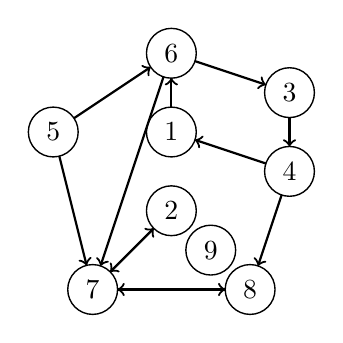
\begin{tikzpicture}[scale=0.5]
   \tikzset{EdgeStyle/.style={->}}
   \Vertex[x=0 ,y=0]{1}
   \Vertex[x=3,y=1]{3}
   \Vertex[x=3 ,y=-1]{4}
   \Vertex[x=0 ,y=2]{6}
   \Vertex[x=0 ,y=-2]{2}
   \Vertex[x=-2 ,y=-4]{7}
   \Vertex[x=2 ,y=-4]{8}
   \Vertex[x=-3 ,y=0]{5}
   \Vertex[x=1 ,y=-3]{9}
   \Edge(6)(3)
   \Edge(3)(4)
   \Edge(4)(1)
   \Edge(1)(6)
   \Edge(4)(8)
   \Edge(6)(7)
   \Edge(2)(7)
   \Edge(7)(2)
   \Edge(7)(8)
   \Edge(8)(7)
   \Edge(5)(6)
   \Edge(5)(7)
\end{tikzpicture}

Initially $H=G$
\end{minipage}
\hfill
\minipage{0.24\textwidth}
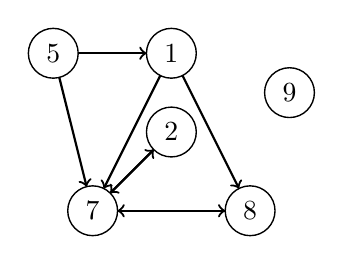
\begin{tikzpicture}[scale=0.5]
   \tikzset{EdgeStyle/.style={->}}
   \Vertex[x=0 ,y=0]{1}
   \Vertex[x=0 ,y=-2]{2}
   \Vertex[x=-2 ,y=-4]{7}
   \Vertex[x=2 ,y=-4]{8}
   \Vertex[x=-3 ,y=0]{5}
   \Vertex[x=3 ,y=-1]{9}
   \Edge(1)(8)
   \Edge(1)(7)
   \Edge(2)(7)
   \Edge(7)(2)
   \Edge(7)(8)
   \Edge(8)(7)
   \Edge(5)(1)
   \Edge(5)(7)
\end{tikzpicture}

After first contraction

when $P=(1,6,3,4)$

and $w=1$
\endminipage\hfill
\minipage{0.24\textwidth}
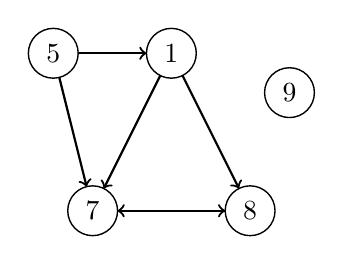
\begin{tikzpicture}[scale=0.5]
   \tikzset{EdgeStyle/.style={->}}
   \Vertex[x=0 ,y=0]{1}
   \Vertex[x=-2 ,y=-4]{7}
   \Vertex[x=2 ,y=-4]{8}
   \Vertex[x=-3 ,y=0]{5}
   \Vertex[x=3 ,y=-1]{9}
   \Edge(1)(8)
   \Edge(1)(7)
   \Edge(7)(8)
   \Edge(8)(7)
   \Edge(5)(1)
   \Edge(5)(7)
\end{tikzpicture}

After second contraction

when $P=(1,8,7,2)$

and $w=7$
\endminipage\hfill
\minipage{0.24\textwidth}
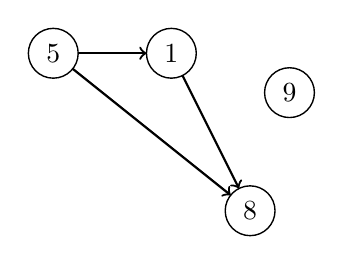
\begin{tikzpicture}[scale=0.5]
   \tikzset{EdgeStyle/.style={->}}
   \Vertex[x=0 ,y=0]{1}
   \Vertex[x=2 ,y=-4]{8}
   \Vertex[x=-3 ,y=0]{5}
   \Vertex[x=3 ,y=-1]{9}
   \Edge(1)(8)
   \Edge(5)(1)
   \Edge(5)(8)
\end{tikzpicture}

After third contraction

when $P=(1,8,7)$

and $w=8$
\endminipage\hfill

\caption{Example of finding the strongly connected components graph}
\label{high_figure}
\end{figure}
\label{high_example}
\end{example}

\subsubsection*{Gabow's implementation}

The implementations of the high level algorithm by Purdom and Munro were not efficient. Therefore Tarjan's algorithm was used instead. But then Gabow found an efficient linear time implementation of the high level algorithm using only two stacks $S$ and $B$ and DFS. The stack $S$ contains the original sequence of vertices in $P$ as visited by DFS, i.e. the whole path without removing contracted vertices. While the stack $B$ contains the boundaries between contracted vertices, i.e. the positions of vertices in S that are left in $P$ after contraction. So if $P=(v_1, v_2,...v_k)$ then $k$ is at the top of $B$ and for all $i = 1,...k-1$ we have $v_i=\{ S[j] : B[i] \leq j < B[i+1] \}$, i.e. the vertex $v_i$ represents all contracted vertices that are strongly connected.

We assume all $n=|V|$ vertices of $G$ are indexed from $1$ to $n$. In addition to stacks $S$ and $B$, an array/list $I[1\ldots n]$ stores the position in the stack $S$ for each vertex, or the index of the strongly connected component it belongs to.  More specifically for a vertex $v$, $I[v] = 0$ if $v$ has not been in $P$ yet, $I[v]=j$ for some integer $j$ if $v$ is currently in $P$ and $S[j]=v$, finally $I[v]=c$ if the strongly connected component of $v$ has been completed and its index is $c$. Note, we assign indices larger than $n$ to strongly connected components, so there is no confusion between vertex's stack position $j$ in $S$ and component index $c$.

Now the algorithm performs DFS of the given graph $G$, while maintaining $S$, $B$ and $I$. When a vertex $v$ is visited by DFS it is pushed onto $S$ and its position in $S$ is pushed onto $B$. We push the position of $v$ in $S$ to $B$, because $v$ is now on the path $P$ and is not (yet) strongly connected with the previously visited vertex. The reason for that is that this is the first time visiting $v$. Therefore we have to push its position (boundary) onto $B$.

When a vertex, $w$, that is already visited is discovered again by DFS, say $P=v_1,v_2,...v_k$ and $w=v_i$, we have found a cycle. Therefore all the vertices $v_{i+1},...v_k$ visited after $w$ and $w$ itself are strongly connected. So we contract them to a single vertex $v_i=\{ S[j] : B[i] \leq j < B[i+1] \}$. To do that pop off positions (boundaries) of all vertices after $w$ by just popping them of until $B[top(b)] \leq I[w]$. Thus only boundaries vertex positions in $S$ from a found strongly connected component are maintained on $B$.

After processing all the edges for each vertex $v$ and returning from recursive calls, we check if a vertex's, $v$, position is at the top of the stack $B$. If it is, then we have found a complete strongly connected component. It consists of $v$ and all vertices on $S$ after $v$, because we have found all reachable vertices from $v$ and all the vertices left on $S$ are strongly connected to $v$, since its position is at the top of $B$. So we just pop all the vertices before $v$ from S and add them to a new strongly connected component. Once this modified DFS is finished we have found all strongly connected components of $G$ and each vertex $v$ of $G$ is assigned its strongly connected components index.

\subsubsection*{Pseudo-code}

\begin{lstlisting}[language=Ruby]
    def SCC(G)
S1:   Create an empty stack S
S2:   Create an empty stack B
S3:   Create a list I marking all vertices as unvisited

S4:   for each yet undiscovered vertex v
S5:     SCC_DFS(G, v)
      end
    end

     def SCC_DFS(G, v)  
D1:    Push v onto S
D2:    Push top(S) on B
  
D3:    for each vertex w adjacent to v
D4:      if w is not discovered
D5:        SCC_DFS(G, w)
D6:      else
           # Pop all positions of vertices discovered after w from B
D7:        while I[w] < B[top(B)] do
D8:          pop(B)
           end
         end
       end
  
       # if position of v in S is at top of B
D9:    if I[v] = B[top(B)] then
D11:     pop(B)
D12:     Pop all vertices w after v from S
D13:     Mark all w as in the same strongly connected component as v
       end
     end
\end{lstlisting}

\begin{example}

Below is given an example of executing the Gabow's algorithm on the graph $G$ in example \ref{SCC_example} to find its strongly connected components. The state of $S$, $B$ and $I$ is given at the same moments as in example \ref{high_example}, and at the moments when returning from recursive call for a vertex $v$ its position is at the top of the stack $B$. Note, processing of vertices 5 and 9 ends almost immediately, as they have only outgoing edges or no edges at all, respectively. Thus their steps are combined in the example.

\begin{figure}[h]

\begin{minipage}[h]{0.24\textwidth}
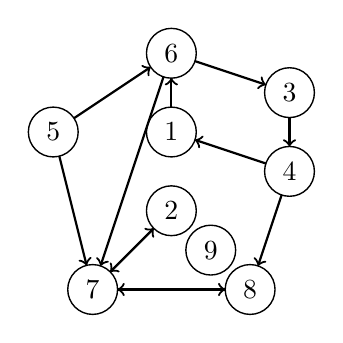
\begin{tikzpicture}[scale=0.5]
   \tikzset{EdgeStyle/.style={->}}
   \Vertex[x=0 ,y=0]{1}
   \Vertex[x=3,y=1]{3}
   \Vertex[x=3 ,y=-1]{4}
   \Vertex[x=0 ,y=2]{6}
   \Vertex[x=0 ,y=-2]{2}
   \Vertex[x=-2 ,y=-4]{7}
   \Vertex[x=2 ,y=-4]{8}
   \Vertex[x=-3 ,y=0]{5}
   \Vertex[x=1 ,y=-3]{9}
   \Edge(6)(3)
   \Edge(3)(4)
   \Edge(4)(1)
   \Edge(1)(6)
   \Edge(4)(8)
   \Edge(6)(7)
   \Edge(2)(7)
   \Edge(7)(2)
   \Edge(7)(8)
   \Edge(8)(7)
   \Edge(5)(6)
   \Edge(5)(7)
\end{tikzpicture}

$I=[0, 0, 0, 0, 0, 0, 0, 0, 0]$

$S=[]$

$B=[]$

\end{minipage}
\hfill
\minipage{0.24\textwidth}
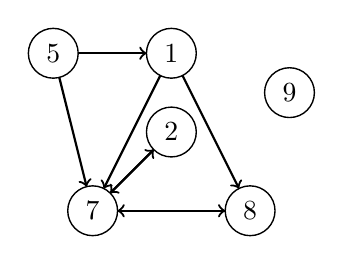
\begin{tikzpicture}[scale=0.5]
   \tikzset{EdgeStyle/.style={->}}
   \Vertex[x=0 ,y=0]{1}
   \Vertex[x=0 ,y=-2]{2}
   \Vertex[x=-2 ,y=-4]{7}
   \Vertex[x=2 ,y=-4]{8}
   \Vertex[x=-3 ,y=0]{5}
   \Vertex[x=3 ,y=-1]{9}
   \Edge(1)(8)
   \Edge(1)(7)
   \Edge(2)(7)
   \Edge(7)(2)
   \Edge(7)(8)
   \Edge(8)(7)
   \Edge(5)(1)
   \Edge(5)(7)
\end{tikzpicture}

After first contraction,

when $P=(1,6,3,4)$

and $w=1$,

$I=[1, 0, 3, 4, 0, 2, 0, 0, 0]$

$S=[1, 3, 4, 6]$

B=[1, 2, 3, 4] to B=[1]
\endminipage\hfill
\minipage{0.26\textwidth}
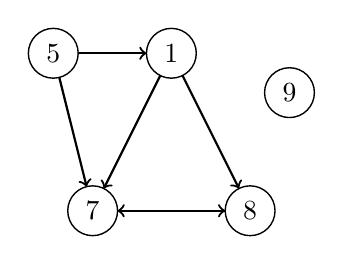
\begin{tikzpicture}[scale=0.5]
   \tikzset{EdgeStyle/.style={->}}
   \Vertex[x=0 ,y=0]{1}
   \Vertex[x=-2 ,y=-4]{7}
   \Vertex[x=2 ,y=-4]{8}
   \Vertex[x=-3 ,y=0]{5}
   \Vertex[x=3 ,y=-1]{9}
   \Edge(1)(8)
   \Edge(1)(7)
   \Edge(7)(8)
   \Edge(8)(7)
   \Edge(5)(1)
   \Edge(5)(7)
\end{tikzpicture}

After second contraction,

when $P=(1,8,7,2)$

and $w=7$,

$I=[1, 7, 3, 4, 0, 2, 6, 5, 0]$

$S=[1, 3, 4, 6, 8, 7, 2]$

B=[1, 5, 6, 7] to B=[1, 5, 6]
\endminipage\hfill
\minipage{0.24\textwidth}
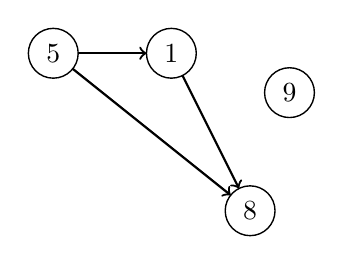
\begin{tikzpicture}[scale=0.5]
   \tikzset{EdgeStyle/.style={->}}
   \Vertex[x=0 ,y=0]{1}
   \Vertex[x=2 ,y=-4]{8}
   \Vertex[x=-3 ,y=0]{5}
   \Vertex[x=3 ,y=-1]{9}
   \Edge(1)(8)
   \Edge(5)(1)
   \Edge(5)(8)
\end{tikzpicture}

After third contraction,

when $P=(1,8,7)$

and $w=8$,

$I=[1, 7, 3, 4, 0, 2, 6, 5, 0]$

$S=[1, 3, 4, 6, 8, 7, 2]$

$B=[1, 5, 6]$ to $B=[1, 5]$
\endminipage\hfill

\vspace*{2\baselineskip}

\minipage{0.33\textwidth}
After we are done with vertex 8:

$I=[1, 10, 3, 4, 0, 2, 10, 10, 0]$

$S=[1, 3, 4, 6]$

$B=[1]$
\endminipage\hfill
\minipage{0.33\textwidth}
After done with vertex 1:

$I=[11, 10, 11, 11, 0, 11, 10, 10, 0]$

$S=[]$

$B=[]$
\endminipage\hfill
\minipage{0.33\textwidth}
End after processing 5 and then 9:

$I=[11, 10, 11, 11, 12, 11, 10, 10, 13]$

S=[5] to S=[] to S=[9] to S=[]

B=[1] to B=[] to B=[1] to B=[]
\endminipage\hfill


\caption{Example of finding the strongly connected components of a graph using Gabow's algorithm}
\end{figure}
\end{example}

\begin{theorem}
Gabow's algorithm finds the strongly connected components of a directed graph $G=(V,E,ends)$ in linear time and space.
\end{theorem}

\begin{proof}
We will prove the first part of the theorem by proving that Gabow's algorithm is a valid implementation of the high level algorithm.
An implementation of the high level algorithm must specify how a path $P=(v_1,v_2,...,v_k)$ is grown. More specifically how it chooses an unprocessed vertex $w$ adjacent to $v_k$ to grow $P$. When $w$ is added to $P$ as the last new vertex, we say that $w$ is activated. Moreover we say that the most active vertex is the currently activated vertex, i.e we order active vertices in their order of activation. Now to choose the next unprocessed vertex $w$ adjacent to $v_k$, let $v$ be the most active vertex. If there is an unprocessed vertex $w$ adjacent to $v$ pick it. If $v$ does not have any unprocessed adjacent vertices left, then deactivate $v$. If this makes all vertices of $v_k$ inactive, then make a strongly connected component from all vertices of $v_k$ and remove it from $P$. This correctly implements the high-level algorithm, because the most active vertex $v$ always belongs to the last vertex $v_k$ of $P$. Notice the activation mechanism mimics recursive DFS.

Now we need to prove that SCC implements the above version of the high level algorithm. We do this by the number of executed statements in SCC, i.e. the number of DFS iterations. If there are no vertices and thus no DFS iterations, the algorithm just returns an empty list, which is correct since there are no strongly connected components in an empty graph. Now assume the algorithm works for $k$ iterations and we must check it for $k+1$ iterations.

When we call SCC\_DFS in line S5 after $k$ iterations, by the inductive assumption for all unvisited vertices $u$ we have $I[u]=0$, and for all visited vertices $z$ we have $I[z] > n$, since we have found and completed all strongly connected components for all vertices. Moreover $P$ and thus $S$ and $B$ are empty, as we are just starting a new path. During the loop at D3 (excluding recursion), $v$ is the most active vertex, since we have just added it to $P$ or deactivated vertices after $v$. In D4 a vertex $w$ is not yet visited, if $I[w]=0$. If $0 < I[w] \leq n$, let $i=I[w]$  then D5 contracts a cycle $(S[i],S[i+1],...S[top(S)])$ or does nothing if it is already contracted, because it pops off positions of all vertices after $w$ by just popping them of until $B[top(b)] \leq I[w]$. If $I[w] > n$ then the component containing $w$ has been deleted and D5 again does nothing.

At D9 we have processed all adjacent vertices to $v$ and check if vertex's $v$ position is at the top of the stack $B$. Assume it is, then it means that we have contracted all vertices on $P$ after $v$ in some combinations of cycles and/or removed the rest of them that are not in those cycles by completing their strongly connected components beforehand. Hence we have found a strongly connected component consisting of of $v$ and all vertices on $S$ after $v$, which the algorithm pops of from the stack $S$ and adds to a new strongly connected component. So after processing the initial vertex we assigned component indices to all visited vertices and have emptied $P$, $S$ and $B$ again. This completes the proof  of the first part of the theorem.

Proving second part of the theorem is relatively straightforward, if the given graph $G$ is stored using adjacency lists. Note that every vertex is pushed (when visited) and popped (when added to a strongly connected component or when contracted) from each stack S and B exactly once and every edge is examined exactly once, too. Thus the algorithm spends constant time and space for each vertex or edge. Therefore it is linear in time and space.
\end{proof}

\section{Parallel algorithm}

All three standard serial algorithms for finding strongly connected components are not well suited for parallelism. It is because they are based on DFS, which is hard to parallelise. In 1985 Reif proved that DFS where adjacent vertices of a vertex are visited in fixed order is P-complete, thus suggesting that it is inherently sequential \cite{reif1985depth}. The approach of executing a standard serial algorithm with different starting conditions is not well suited either. Because, although we can pick a different starting vertices for say Gabow's algorithm iterations, it will be of no use when the graph has very few large strongly connected components. Therefore a completely different approach is needed.

In 2000 a parallel algorithm, called forwards-backwards algorithm, for identifying strongly connected components of a directed graph for shared memory model was developed \cite{fleischer2000identifying}. It achieves parallelism by splitting the graph into four disjoint partitions - intersection of forwards and backwards reachable vertices for some vertex (its strongly connected component), the rest of backwards and the rest of forwards reachable vertices and the rest of vertices. Then the algorithm is recursively applied to the three parts. Furthermore adding a simple trim step to eliminate vertices without incoming or outgoing edges improves performance significantly \cite{mclendon2005finding}. Later the limited performance and poor scaling for large real-world graphs was improved as well by adding various extensions like parallel trimming, two-phase parallelisation and fast detection of size 2 strongly connected components \cite{hongtechnical}.

\subsection{Forwards-backwards algorithm}

This subsection is based on the paper\cite{fleischer2000identifying}. First we will formally define forwards and backwards reachable vertices. 

\begin{definition}[Forwards reachable]
Let $G=(V, E, ends)$ be a directed graph and $v,w \in V$ be two vertices of $G$, then $w$ is $forwards \ reachable$ from $v$ if there is a path from $v$ to $w$. Denote the set of forwards reachable vertices from $v$ in $G$ by $FW_G(v)$.
\end{definition}

\begin{definition}[Backwards reachable]
Let $G=(V, E, ends)$ be a directed graph and $v,w \in V$ be two vertices of $G$, then $w$ is $backwards \ reachable$ from $v$ if there is a path from $w$ to $v$. Denote the set of backwards reachable vertices from $v$ in $G$ by $BW_G(v)$.
\end{definition}

The following lemma gives the reason why finding forwards and backwards reachable vertices helps finding strongly connected components.

\begin{lemma}
Let $G=(V, E, ends)$ be a directed graph and $v \in V$ be a vertex of $G$. Then the subgraph induced by vertices of $FW_G(v) \cap BW_G(v)$ is the strongly connected component $SCC_G(v)$ of $G$ containing $v$.
\label{fw_bw_l1}
\end{lemma}

\begin{proof}
Let $w$ be any vertex of $G$. Then

$w \in FW_G(v) \cap BW_G(v) \Leftrightarrow$

$w$ is both forwards and backwards reachable from $v$ $\Leftrightarrow$

There is a path from $v$ to $w$ and a path from $w$ to $v$ $\Leftrightarrow$

$v$ and $w$ are strongly connected $\Leftrightarrow$

$w$ is in  $SCC_G(v)$.

Thus $FW_G(v) \cap BW_G(v)$ and $SCC_G(v)$ contain the same vertices, therefore the subgraph induced by vertices of $FW_G(v) \cap BW_G(v)$ is the strongly connected component $SCC_G(v)$ of $G$ containing $v$. 
\end{proof}

\begin{definition}[Remainder]
Let $G=(V, E, ends)$ be a directed graph and $v \in V$ be a vertex of $G$. The $remainder$ of $v$ in $G$ is the set of vertices $Rem_G(v)=V \setminus (FW_G(v) \cup BW_G(v))$, i.e. the vertices that are neither forwards or backwards reachable from $v$.
\end{definition}

Now we establish that any strongly connected compoenent is in one of the three disjoint partitions.

\begin{lemma}
Let $G=(V, E, ends)$ be a directed graph and $v \in V$ be a vertex of $G$. Then any other strongly connected component of $G$ apart from $SCC_G(v)$ is in exactly one of subgraphs induced by $FW_G(v) \setminus BW_G(v)$, $BW_G(v) \setminus FW_G(v)$) or $Rem_G(v)$.
\label{fw_bw_l2}
\end{lemma}

\begin{proof}
Let $u$ and $w$ be two vertices of the same strongly connected component in $G$ that is not $SCC_G(v)$. Now since $u$ and $w$ are in the same strongly connected component there is a path from $u$ to $w$ and a path from $w$ to $u$.

If $u \in FW_G(v)$ then there is a path from $v$ to $u$, thus there is a path from $v$ to $w$ (through $u$) and so $w \in FW_G(v)$. Similarly if $w \in FW_G(v)$ then $u \in FW_G(v)$. Therefore $w \in FW_G(v) \Leftrightarrow u \in FW_G(v)$. Similar argument shows that $w \in BW_G(v) \Leftrightarrow u \in BW_G(v)$.
Thus $w \in Rem_G(v) \Leftrightarrow u \in Rem_G(v)$, as $Rem_G(v)=V \setminus (FW_G(v) \cup BW_G(v))$.

Now since $u$ and $w$ are in different strongly connected component that $SCC_G(v)$, then $u,v \not \in FW_G(v) \cap BW_G(v)$. And so both $u$ and $v$ are in exactly one of $FW_G(v) \setminus BW_G(v)$, $BW_G(v) \setminus FW_G(v)$) or $Rem_G(v)$, as they are disjoint. So all vertices of a strongly connected component that is not $SCC_G(v)$ are in exactly one of the tree sets. Therefore any other strongly connected component of $G$ apart from $SCC_G(v)$ is in exactly one of subgraphs induced by $FW_G(v) \setminus BW_G(v)$, $BW_G(v) \setminus FW_G(v)$) or $Rem_G(v)$.
\end{proof}

Now the algorithm itself as described before is fairly simple. We pick a vertex $v$ in $G$, then find $FW_G(v)$ and $BW_G(v)$ by using DFS or BFS on $v$. To find $BW_G(v)$ we at very beginning of the algorithm compute the reverse graph of $G$. Then we calculate $FW_G(v) \cap BW_G(v)$ and add it as a strongly connected component. After that just recursively repeat the same algorithm in parallel on $FW_G(v) \setminus BW_G(v)$, $BW_G(v) \setminus FW_G(v)$) and $Rem_G(v)$, since any other strongly connected component of $G$ is in exactly one of those vertex set induced graphs.

It achieves parallelism by splitting the graph into four disjoint partitions - intersection of forwards and backwards reachable vertices for some vertex (its strongly connected component), the rest of backwards and the rest of forwards reachable vertices and the rest of vertices. Then the algorithm is recursively applied to the three parts

\subsubsection*{Pseudo-code}

\begin{lstlisting}[language=Ruby, mathescape]
def FW-BW(G, SCC)

  if G has no vertices
    return

  v = any vertex of G
  $FW_G(v) = $ forwards reachable vertices from v in G
  $BW_G(v) = $ backwards reachable vertices from v in G
  $S = FW_G(v) \cap BW_G(v)$
  Add S to SCC
  
  do in parallel
    FW-BW(InducedGraph($FW_G(v) \setminus BW_G(v)$), SCC)
    FW-BW(InducedGraph($BW_G(v) \setminus FW_G(v)$), SCC)
    FW-BW(InducedGraph($G \setminus (FW_G(v) \cup BW_G(v))$, SCC)
end
\end{lstlisting}

\begin{example}
An example of executing the forwards-backwards algorithm on the graph $G$ in example \ref{SCC_example} to find its strongly connected components. The algorithm say picks vertex 1 as the starting point, then $BW_G(v) = \{1, 6, 3, 4, 5\}$, $FW_G(v) = \{1, 6, 3, 4, 8, 7, 2\}$, so $S=\{1,6,3,4\}$. After that recursively apply the algorithm on $BW_G(v) \setminus FW_G(v) = \{5\}$, $FW_G(v) \setminus BW_G(v) = \{2, 7, 8\}$ and $Rem_G(v)=\{9\}$. All three of which turn out to be full strongly connected components by themselves, so we are done and have found all strongly connected components of $G$.

\begin{figure}[!htb]
			\minipage{0.32\textwidth}
  			\SetVertexNormal[Shape      = circle,
                 FillColor  = blue!20,
                 LineWidth  = 2pt]
\SetUpEdge[lw         = 3pt,
           color      = black,
           labelcolor = white,
           labeltext  = red,
           labelstyle = {sloped,draw,text=blue}]
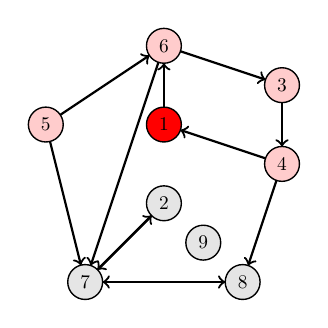
\begin{tikzpicture}[scale = 0.5]
   \tikzset{EdgeStyle/.style={->}}
   \tikzset{VertexStyle/.append  style={fill=red, scale = 0.7}}
   \Vertex[x=0 ,y=0]{1}
   \tikzset{VertexStyle/.append  style={fill=red!20}}
   \Vertex[x=3,y=1]{3}
   \Vertex[x=3 ,y=-1]{4}
   \Vertex[x=0 ,y=2]{6}
   \tikzset{VertexStyle/.append  style={fill=gray!20}}
   \Vertex[x=0 ,y=-2]{2}
   \Vertex[x=-2 ,y=-4]{7}
   \Vertex[x=2 ,y=-4]{8}
   \tikzset{VertexStyle/.append  style={fill=red!20}}
   \Vertex[x=-3 ,y=0]{5}
   \tikzset{VertexStyle/.append  style={fill=gray!20}}
   \Vertex[x=1 ,y=-3]{9}
   \Edge(6)(3)
   \Edge(3)(4)
   \Edge(4)(1)
   \Edge(1)(6)
   \Edge(4)(8)
   \Edge(6)(7)
   \Edge(2)(7)
   \Edge(7)(2)
   \Edge(7)(8)
   \Edge(8)(7)
   \Edge(5)(6)
   \Edge(5)(7)
\end{tikzpicture}
\center{Backwards reachable}
			\endminipage\hfill
			\minipage{0.32\textwidth}
  			\SetVertexNormal[Shape      = circle,
                 FillColor  = blue!20,
                 LineWidth  = 2pt]
\SetUpEdge[lw         = 3pt,
           color      = black,
           labelcolor = white,
           labeltext  = red,
           labelstyle = {sloped,draw,text=blue}]
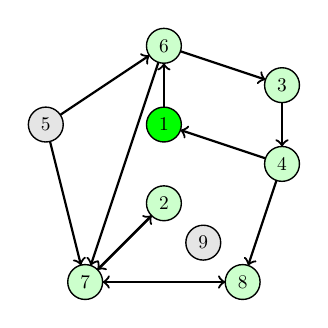
\begin{tikzpicture}[scale=0.5]
   \tikzset{EdgeStyle/.style={->}}
   \tikzset{VertexStyle/.append  style={fill=green, scale=0.7]}}
   \Vertex[x=0 ,y=0]{1}
   \tikzset{VertexStyle/.append  style={fill=green!20}}
   \Vertex[x=3,y=1]{3}
   \Vertex[x=3 ,y=-1]{4}
   \Vertex[x=0 ,y=2]{6}
   \tikzset{VertexStyle/.append  style={fill=green!20}}
   \Vertex[x=0 ,y=-2]{2}
   \Vertex[x=-2 ,y=-4]{7}
   \Vertex[x=2 ,y=-4]{8}
   \tikzset{VertexStyle/.append  style={fill=gray!20}}
   \Vertex[x=-3 ,y=0]{5}
   \tikzset{VertexStyle/.append  style={fill=gray!20}}
   \Vertex[x=1 ,y=-3]{9}
   \Edge(6)(3)
   \Edge(3)(4)
   \Edge(4)(1)
   \Edge(1)(6)
   \Edge(4)(8)
   \Edge(6)(7)
   \Edge(2)(7)
   \Edge(7)(2)
   \Edge(7)(8)
   \Edge(8)(7)
   \Edge(5)(6)
   \Edge(5)(7)
\end{tikzpicture}
\center{Forwards reachable}
			\endminipage\hfill
			\minipage{0.32\textwidth}
  			\SetVertexNormal[Shape      = circle,
                 FillColor  = blue!20,
                 LineWidth  = 2pt]
\SetUpEdge[lw         = 3pt,
           color      = black,
           labelcolor = white,
           labeltext  = red,
           labelstyle = {sloped,draw,text=blue}]
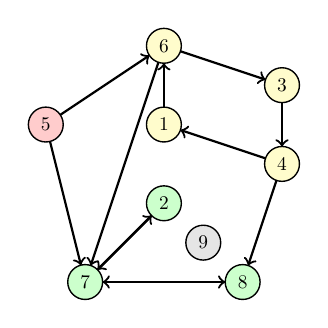
\begin{tikzpicture}[scale=0.5]
   \tikzset{EdgeStyle/.style={->}}
   \tikzset{VertexStyle/.append  style={fill=yellow!20, scale=0.7]}}
   \Vertex[x=0 ,y=0]{1}
   \tikzset{VertexStyle/.append  style={fill=yellow!20}}
   \Vertex[x=3,y=1]{3}
   \Vertex[x=3 ,y=-1]{4}
   \Vertex[x=0 ,y=2]{6}
   \tikzset{VertexStyle/.append  style={fill=green!20}}
   \Vertex[x=0 ,y=-2]{2}
   \Vertex[x=-2 ,y=-4]{7}
   \Vertex[x=2 ,y=-4]{8}
   \tikzset{VertexStyle/.append  style={fill=red!20}}
   \Vertex[x=-3 ,y=0]{5}
   \tikzset{VertexStyle/.append  style={fill=gray!20}}
   \Vertex[x=1 ,y=-3]{9}
   \Edge(6)(3)
   \Edge(3)(4)
   \Edge(4)(1)
   \Edge(1)(6)
   \Edge(4)(8)
   \Edge(6)(7)
   \Edge(2)(7)
   \Edge(7)(2)
   \Edge(7)(8)
   \Edge(8)(7)
   \Edge(5)(6)
   \Edge(5)(7)
\end{tikzpicture}
\center{Disjoint parts and S}
			\endminipage\hfill
			\label{fw_bw_fig}
			\caption{Example of forwards-backwards algorithm execution}
		\end{figure}
		
\end{example}

complexity, discussion on efficiency.

\begin{theorem}
Let $G=(V, E, ends)$ be a directed graph. Then the forwards-backwards algorithm (FW-BW) correctly finds all strongly connected components of $G$.
\end{theorem}
\begin{proof}
It is a direct consequence of lemmas \ref{fw_bw_l1} and \ref{fw_bw_l2}, because we find one strongly connected component using results from lemma \ref{fw_bw_l1}, then divide the problem in 3 disjoint parts using lemma \ref{fw_bw_l2} and recursively solve that.
\end{proof}

\begin{theorem}
Let $G=(V, E, ends)$ be a directed graph in which all vertex degrees are bounded by a constant. Then the forwards-backwards algorithm (FW-BW) has expected serial time complexity $O(n \, logn)$ where $n=|V|$.
\end{theorem}

The proof of this theorem is not given as it is too long and complicated and so outside the scope of this text. This theorem means that forwards-backwards algorithm is not much more inefficient that the Gabow's algorithm, so it is worthwhile to parallelise. Moreover it should achieve good parallelism, since each partition produces three new partitions and so the number of partitions that can be processed in independently in parallel grows quickly \cite{hongtechnical}, especially for graphs that have many similar size strongly connected components.

Unfortunately this is not always the case. Assume we have a real world network graph (e.g a graph of a social network). These usually have one strongly connected component that is very large. This causes load imbalance. Moreover, it is very likely that a vertex from it is picked first. So while it is identified by one processor all others stay idle. This issue with real world network graphs can be solved by adding various optimizations such as parallel trimming, two-phase parallelisation and fast detection of size 2 strongly connected component \cite{hongtechnical}.

We will closer examine the parallel trimming optimization, as it is the most effective and not only for real world network graphs.

\subsection{Parallel trim step}

The trim step allows to identify trivial strongly connected components (those with only one vertex), because these have only incoming or outgoing edges after other trimmed vertices are removed. Therefore we can easily identify them by looking how many incoming and outgoing edges they have. If a vertex after other trimmed vertices are removed has zero incoming (in-degree) or zero outgoing edges (out-degree), then it is a trivial strongly connected component and can be trimmed. Note that trimming is applied iteratively since it can enable further trimming \cite{hongtechnical}.

\subsubsection*{Pseudo-code}

\begin{lstlisting}[language=Ruby]
def Trim(G, SCC)
  do
    for each vertex v in G
      if in-deg(G, v) = 0 or out-deg(G, v) = 0
        Add v to SCC
        Remove v and all its edges from G
  while G is changed
end
\end{lstlisting}

Note this can be implemented without actually modifying the graph and avoiding performance overhead by just keeping track of how many incoming and outgoing edges each vertex has and just marking the vertices as trimmed and not considering them for trimming again. Then constructing a new graph at the end without all trimmed vertices. Note we can parallelise the inner for-loop of the trim step, because "removal" of a vertex from $G$ only affects the vertices examined after it. So as long as we repeat the outer loop we will trim exactly the same vertices at the end as in serial implementation.

\section{Partial strongly connected components}

Often, instead of computing all strongly connected components of a directed graph $G=(V, E, ends)$, one would like to do that only partially step by step. For example find if two vertices are strongly connected or a strongly connected component of a specific vertex and then do that again for different vertices/vertex while remembering the results of previous computation. Both the Gabow's and forwards-backwards algorithms can be easily modified to achieve this.

For Gabow's algorithm to find the strongly connected component of a vertex $v$ we execute it starting at that vertex and do only one iteration of it. At the end of that iteration we have found $SCC_G(v)$ and possibly other strongly connected components. More specifically, all of the strongly connected components that are forwards reachable from $v$. This intermediate result can be saved by simply keeping the list $I$ of strongly connected component's index each vertex of $G$ belongs to. Note that at the end of each iteration the stacks $S$ and $B$ are empty so we do not need to keep these and all entries in $I$ either mark a vertex as undiscovered or in some strongly connected component. Now whenever we want to find out something about strong connectedness in our graph we just reuse the list $I$. And if some vertex $w$ in question is marked as undiscovered we again execute one iteration of Gabow's algorithm starting at $w$.

For forwards-backwards algorithm we again start at some specific vertex and keep the intermediate results. In this case we must keep track of the disjoint partitions and to which partition each vertex belongs to.

\chapter{Vertex colouring}

\section{Defining vertex colouring}

\begin{definition}[Vertex colouring]
Let $G=(V, E, ends)$ be a graph, then a $vertex \ colouring$ is an assignment of colours to all vertices of $G$ such that every pair of adjacent vertices has distinct colours. 
\end{definition}

We will often use natural numbers instead of real colours, due to simpler use when the number of colours is not small. Thus a $k-colouring$ of a graph $G$ is a function $c: V(G) \leftarrow \{1, 2,..., k\}$ such that $c(v) \not = c(w)$ for all adjacent vertices $v,w$ of $G$.

\begin{example}

An example of a vertex colouring with 4 colours (blue, green, yellow, red) where no two adjacent vertices have the same colour. Note that 4 colours is the minimum due to the complete subgraph (3,4,5,6) with 4 vertices - a graph that has an edge between every pair of distinct vertices, i.e. all possible edges. Moreover, this is not the only valid colouring.

\begin{figure}[h]
\center
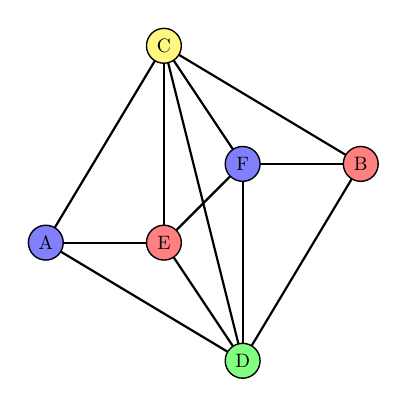
\begin{tikzpicture}[scale=0.5]
   \tikzset{VertexStyle/.append style={scale=0.7}}
   \tikzset{VertexStyle/.append style={fill=yellow!50}}
   \Vertex[x=-1 ,y=4]{C}
   \tikzset{VertexStyle/.append style={fill=green!50}}
   \Vertex[x=1, y = -4]{D}
   \tikzset{VertexStyle/.append style={fill=red!50}}
   \Vertex[x=4 ,y=1]{B}
   \Vertex[x=-1 ,y=-1]{E}
   \tikzset{VertexStyle/.append style={fill=blue!50}}
   \Vertex[x=-4 ,y=-1]{A}
   \Vertex[x=1, y=1]{F}
   \Edge(A)(C)
   \Edge(A)(D)
   \Edge(A)(E)
   \Edge(B)(C)
   \Edge(B)(D)
   \Edge(B)(F)
   \Edge(C)(D)
   \Edge(C)(E)
   \Edge(C)(F)
   \Edge(D)(E)
   \Edge(D)(F)
   \Edge(E)(F)
\end{tikzpicture}
\caption{An example of a valid vertex colouring}
\end{figure}
\label{VC_example}
\end{example}

The problem we will look at is finding a vertex $k-colouring$ for some graph $G$ or establishing that $G$ cannot be coloured with $k$ colours for some positive integer $k$. It has many various applications, especially in scheduling and clustering type problems. One of the most famous examples is colouring a map, where the countries/regions of a map are vertices and there is an edge between them if they have a common border in the map. Vertex colouring of such a graph gives a way to colour the map, so that countries/regions with common borders have different colours for better visibility.

Another common application is solving scheduling problems. For example scheduling student's classes so that no student has two at the same time. In this case vertices are the classes and there is an edge between them if some student is taking both of them, so the colours are timetable slots. Another scheduling example is compiler optimization - scheduling the use of registers, i.e. two variables whose lifetime overlaps cannot be placed in the same register. So variables are vertices and registers are colours \cite{skiena504algorithm}. Other brief examples are finding if a graph is bipartite or planar \cite{skiena504algorithm}, placing security cameras in an arts gallery, round-robin sports scheduling, aircraft scheduling and assigning frequencies to radio stations \cite{ahmed2012applications}.

Unfortunately vertex colouring of general graphs is hard. In fact, it is NP-complete. So at the moment there is no known solution that has polynomial worst-case time complexity. The proof, which we will not cover here, converts a vertex colouring problem to a 3-SAT satisfiability problem, which is proven to be NP-complete \cite{gibbons1985algorithmic}. Thus, since vertex colouring is at least as hard as 3-SAT satisfiability problem, it has to be NP-complete.

\section{Serial algorithms}

Since vertex colouring is hard, many vertex colouring solutions are heuristic and are meant to find an approximation for the minimum number $k$ of colours for a graph to be $k-colourable$. Thus those approaches do not always give an optimal answer. Note that finding the minimum number of colours and whether a graph is $k-colourable$ for some positive integer $k$ are very similar problems and an algorithm for one gives an algorithm for another. Because, if we know that a graph can be coloured at minimum with $k$ colours and we have such a colouring, then we know that a graph cannot be coloured with less than $k$ colours and we already have a colouring with at least $k$ colours. For the other way around we just check if there is a colouring for $1,2,3,..$ colours until we find one, the process clearly stops since a graph with $v$ vertices can be clearly coloured with $v$ colours.

Despite that in this text we are only interested in exact deterministic algorithms for finding a vertex $k-colouring$ for some graph $G$ or establishing that $G$ cannot be coloured with $k$ colours for some positive integer $k$.

\subsection{Brute force}

Now we will briefly consider one very simple way of finding a $k-colouring$ for some graph $G$ and a positive integer $k$. It is a brute force search - we look at every possible assignment of $k$ colours to the vertices of a graph and check if no two adjacent vertices have the same colour. We can generate all the possible colourings recursively and do not recurse further for the partial colourings that are already invalid. 

\subsubsection*{Pseudo-code}

\begin{lstlisting}[language=Ruby]
def IsValidColouring(G, v, colouring)
  for each vertex w adjacent to v do
      if colouring(v) = colouring(w) then
        return false
      end
  end
        
  return true
end

def ColourVerticesBF(G, colouring)

  if colouring has coloured all vertices of G then
    return colouring
  end
  
  pick next uncoloured vertex v  
  
  for each colour c
    colouring(v) = c
    if IsValidColouring(G, v, colouring) then
      ColourVerticesBF(G, colouring)
    end
  end
end
\end{lstlisting}

This method is very inefficient and impractical, because if $G$ has $v$ vertices and we use $k$ colours for each vertex, then there are $v^k$ possible colourings. Moreover, if $G$ cannot be $k-coloured$ we have to check all of these colourings, thus such an algorithm has an exponential worst case time complexity. Therefore we will not look into this method in more detail. Therefore we present an algorithm that has the same worst case time complexity, but is much more efficient in practice. It is the backtracking algorithm.

\subsection{Backtrack}

Since vertex colouring is NP-complete we cannot do much better than the brute force algorithm, but we still cannot do significantly better. The standard deterministic exact algorithm for vertex colouring is a backtracking solution \cite{skiena504algorithm}. It essentially tries a colouring and backtracks to the last assigned vertex that caused a clash of colours. More precisely it assigns colours one by one to the vertices of a graph $G$ and before assigning a colour $c$ to a vertex $v$ checks if it is still valid. To do that it just considers all adjacent vertices of $v$ and checks that none of them have colour $c$. If after assigning the colour $c$ the colouring is still valid, we just pick the next vertex and try to assign a colour to that. If the colouring is not valid, we backtrack.

We backtrack until the last coloured vertex whose colour is used at least for one other vertex and whose colour is not $k$, assuming  the $k$ colours are numbered from 1 to $k$. We skip vertices whose colour has been assigned only to them, is because they clearly could not have caused a clash anywhere. And we skip vertices whose colour is $k$, because that is the last colour we try, and so that vertex does not have any other options left. When we find such a vertex we just increase its colour by one, check it and repeat the same process. If we do not find such a vertex, it means that we have explored all possible valid colourings and thus there is no colouring with $k$ colours.

\subsubsection*{Pseudo-code}

\begin{lstlisting}[language=Ruby]
def IsValidAssignment(G, v)
  for each vertex w adjacent to v do
    if colour(v) = colour(w) then
      return false
    end
  end
        
  return true
end

def ColourVerticesBT(G)

  while there are uncoloured vertices v do
  
    colour v  with the next colour
    if  IsValidAssignment(G, v) then
      numberOfColours(colour(v)) = numberOfColours(colour(v)) + 1
      pick v to be next vertex
    else
      # backtrack
      while  numberOfColours(colour(v)) == 1 or colour(v) == k do
      
        uncolour v      
      
        if there are no more vertices left to backtrack to then
          return no solutions
        else
          pick v to be the previous vertex
        end
        
      colour v with the next colour
    end
  end    
   
  return the colouring
end
\end{lstlisting}

\begin{theorem}
For a graph $G$ and some positive integer $k$, if $G$ can be $k-coloured$ then the backtracking vertex colouring algorithm finds a valid vertex $k-colouring$ (possibly with even less colours). If $G$ cannot be $k-coloured$ then the algorithm correctly identifies that it is the case.
\end{theorem}

\begin{proof}
We already know that we can find a $k-colouring$ or establish its non-existence by considering all possible colourings. To prove the correctness of the backtracking algorithm we will show that it considers all possible colourings worth exploring. More precisely, only colourings it does not consider are the ones that we know will not yield a solution or will yield a solution only if some other colouring that we are considering will yield a solution. 

Let $v_1,v_2,...,v_n$ be all vertices of $G$ and assume the algorithm is picking the vertices in that order.
Now there are only four different possibilities for some of the colourings to be discarded by the backtracking algorithm. First is when a vertex $v_i$ has just been assigned a colour, but it clashes with a colour of another adjacent vertex $v_j$. More precisely, we assign a colour $c$ to the vertex $v_i$, but there is an adjacent vertex $v_j$ such that $j<i$ and the colour of $v_j$ is $c$. In this case no matter how we colour the rest of vertices $v_{i+1},v_{i+2},...,v_n$, we will not find a solution, because vertices $v_i$ and $v_j$ will still be adjacent and have the same colour $c$. Therefore we can safely backtrack and consider the next colour for $v_i$.

Second, skipping a vertex which is the only vertex of that colour is fine, too. Because no other vertex has the same colour thus changing its colour reduces the number of colours in the current colouring. But if we can complete the colouring with one less colour, then we can clearly complete it using one more. Third, we clearly have to backtrack when we have exhausted all colours of a vertex. Forth, when we backtrack to the first vertex there is no point in trying any other colours than the first one, because we can permute the colours of a colouring in such a way that the first vertex always has the first colour.

Thus we have shown that the backtracking algorithm considers all possible colourings worth exploring. Therefore it is correct.
\end{proof}

\begin{example}

An example of colouring the graph from the example \ref{VC_example} with 4 colours using the backtracking algorithm. In this example we assume that vertices are in alphabetic order, i.e. the backtrack algorithm considers them in the order A, B, C, D, E, F and that the colours are in the order blue, red, yellow, green. We present the search tree of the backtracking algorithm - the tree of the explored colouring assignments. The leaves of the tree are the dead ends where we found a clash of colours. While the right most path is the valid colouring found by the backtracking algorithm.

\begin{figure}[h]

\tikzset{
  treenode/.style = {align=center, inner sep=0pt, text centered, circle, font=\sffamily\bfseries,  text width=1em, font=\sffamily},
  arn_b/.style = {treenode, draw=black, fill=blue!50},
  arn_r/.style = {treenode, draw=black, fill=red!50},
  arn_y/.style = {treenode, draw=black, fill=yellow!50},
  arn_g/.style = {treenode, draw=black, fill=green!50},
}

\center
\begin{tikzpicture}[->,>=stealth',level/.style={sibling distance = 4cm/#1,
  level distance = 1.5cm}] 
\node[arn_b] {A}
  child { node[arn_b]{B}
    child{ node[arn_b]{C} }
    child{ node[arn_r]{C}
      child{ node[arn_b]{D} }
      child{ node[arn_r]{D} }
      child{ node[arn_y]{D}
        child{ node[arn_b]{E} }
        child{ node[arn_r]{E} }
        child{ node[arn_y]{E} }
        child{ node[arn_g]{E}
          child{ node[arn_b]{F} }
          child{ node[arn_r]{F} } 
          child{ node[arn_y]{F} } 
          child{ node[arn_g]{F} } 
        }
      }
    }
  }
  child {node[arn_r]{B}
    child {node[arn_b]{C} }
    child {node[arn_r]{C} }  
    child {node[arn_y]{C}
      child{ node[arn_b]{D} }
      child{ node[arn_r]{D} }
      child{ node[arn_y]{D} }
      child{ node[arn_g]{D}
        child{ node[arn_b]{E} }
        child{ node[arn_r]{E}
          child{ node[arn_b]{F} }      
        } 
      }
    }  
  }

; 
\end{tikzpicture}
\caption{An example of the backtracking algorithm finding a solution}
\end{figure}
\label{VC_example1}
\end{example}

\begin{example}

An example of trying to colour the graph from the example \ref{VC_example} with 3 colours using the backtracking algorithm. Again we assume that vertices are in alphabetic order, i.e. the backtrack algorithm considers them in the order A, B, C, D, E, F and that the colours are in the order blue, red, yellow. And again we present the search tree of the backtracking algorithm. Note that the graph cannot be coloured with 3 colours due to having a complete subgraph of 4 vertices (3,4,5,6). Therefore the backtracking algorithm backtracks back to the first vertex A. Thus it fails and so correctly returns that there are no solutions. So this time all leaves are dead ends of clashing colours.

\begin{figure}[h]

\tikzset{
  treenode/.style = {align=center, inner sep=0pt, text centered, circle, font=\sffamily\bfseries,  text width=1em, font=\sffamily},
  arn_b/.style = {treenode, draw=black, fill=blue!50},
  arn_r/.style = {treenode, draw=black, fill=red!50},
  arn_y/.style = {treenode, draw=black, fill=yellow!50},
  arn_g/.style = {treenode, draw=black, fill=green!50},
}

\center
\begin{tikzpicture}[->,>=stealth',level/.style={sibling distance = 4cm/#1,
  level distance = 1.5cm}] 
\node[arn_b] {A}
  child { node[arn_b]{B}
    child{ node[arn_b]{C} }
    child{ node[arn_r]{C}
      child{ node[arn_b]{D} }
      child{ node[arn_r]{D} }
      child{ node[arn_y]{D}
        child{ node[arn_b]{E} }
        child{ node[arn_r]{E} }
        child{ node[arn_y]{E} }
      }
    }
  }
  child {node[arn_r]{B}
    child {node[arn_b]{C} }
    child {node[arn_r]{C} }  
    child {node[arn_y]{C}
      child{ node[arn_b]{D} }
      child{ node[arn_r]{D} }
      child{ node[arn_y]{D} }
    }  
  }
; 
\end{tikzpicture}
\caption{An example of the backtracking algorithm not finding a solution}
\end{figure}
\end{example}

\begin{theorem}
For a graph $G$ with $n$ vertices and some positive integer $k$, if $G$ can be $k-coloured$ the backtracking algorithm has worst case time complexity of $O(n^k)$
\label{BT_wc}
\end{theorem}

\begin{proof}
The backtracking algorithm does not consider an assignment of colours multiple times, because when backtracking we never consider the previous colour. We always pick the next colour. Therefore the backtracking algorithm is no worse than the brute force algorithm and has the worst case time complexity of $O(k^n)$.

Note that we cannot have a smaller upper bound for the worst case time complexity than $O(k^n)$. To show that we give for any number of colours $k$ an example of a graph to which adding $m$ vertices always means that the number of colourings considered is at least $k^m$. Thus backtracking for such a graph would have worst-case time complexity of at least $O(n^k)$, as it has exponential growth factor of $k$.

Consider the complete graph $K_{k+1}$ with $k+1$ vertices. We already know that it cannot be coloured with $k$ colours, thus we know that the backtracking algorithm will not find a solution and thus will not stop early. So it will keep going until it backtracks to the first vertex it considered. Furthermore, the same holds for any graph $G$ which we get by adding $m$ vertices to $K_{k+1}$. Now add $m$ vertices with no edges to the graph $K_{k+1}$ and assume that the backtracking algorithm considers them before the vertices of $K_{k+1}$. This means that it will consider all possible colourings for the $m$ added vertices, because there are no edges between them and therefore no clashes. Therefore it will explore at least $k^m$ colourings.
\end{proof}

Now lets compare the backtracking algorithm versus the brute force algorithm. The backtracking algorithm considers a colouring and all of its possible colour permutations, because it considers all possible colourings. So for example if we have a graph with 2 vertices and use 2 colours ($1$ and $2$) two of the colourings it will consider $1,1$ and the colouring $2,2$. But this is clearly it is sufficient to consider only one of them, because $1,1$ is a valid colouring if and only if $2,2$ is a valid colouring. Because the only condition is that no two adjacent vertices have the same colour and there is no distinction between different colours. Therefore we can freely permute them.

This is exactly what the backtracking algorithm does for each colour assignment it considers only one of its colour permutations.

\begin{theorem}
The backtracking algorithm does not consider multiple colour assignments that can be obtained from each other by permuting the colours.
\end{theorem}

\begin{proof}
Let $1,2,..,k$ be the $k$ colours and $v_1,v_2,...,v_n$ be vertices, i.e. we just enumerate them. We will refer to a colour assignment as list of colours where the vertex $v_i$ has the $i-th$ element of the list as its colour or 0 if it has no colour assigned yet. So for example if we have a graph with three vertices and $v_1$ has colour 3, and $v_3$ has colour 2, while $v_2$ has no colour. We denote it by $3,0,2$.

We will prove the theorem using induction on the number of vertices with assigned colour. Let $C_1$ be a colour assignment only to the first vertex. The only $C_1$ the backtracking algorithm considers is $C_1=1$, because when we backtrack to the first vertex the algorithm stops and returns no solutions. This is the base case of the induction.

Now assume than for some natural number $n$ any colour assignment on the first $n$ vertices considered by the algorithm is not a permutation of of some other considered colouring assignment. Not let $C_{n+1}$ be a colouring assignment. The algorithm considers it if and only if there is some colouring assignment $C_n$ on the first $n$ vertices considered by the algorithm. By the inductive assumption the colouring assignment $C_n$ is not a permutation of some other considered colouring assignment. Note that if two colourings are not colour permutations of each other, then even after colouring some extra vertices these colourings are still not colour permutations of each other. Therefore $C_{n+1}$ can only be a colouring permutation of an assignment that is obtained from $C_n$ by colouring the $v_{n+1}$ vertex. 

Consider the colour $c$ assigned to the $v_{n+1}$ vertex. If $c$ has been already assigned a vertex $v_i$ for some $i<n$, then $C_{n+1}$ is not a permutation of some other colouring assignment obtained from $C_n$ by colouring the $v_{n+1}$ vertex. Because in these two assignments $v_i$ has the same colour assigned, but $v_{n+1}$ has different colours assigned.

If $c$ has not already been assigned to some vertex, then $c=max(C_n)+1$, where $max(C_n)$ is the largest colour assigned in $C_n$. Because, while backtracking the algorithm backtracks to the previous vertex instead of picking the next colour, when the colour used for the last vertex has not been used before. So once we assign colour $max(C_n)+1$ to $v_{n+1}$ we will not assign any larger colour to it without backtracking to vertex $v_{n}$ and thus considering different assignment from $C_n$ on the first $n$ vertices. Note this also means that every colour smaller than $max(C_n)$ has also been assigned in $C_n$. Therefore if $c$ has not already been assigned to some vertex, the algorithm considers only one possibility for $C_{n+1}$, which clearly is not a colour permutation of the other considered assignments obtained from $C_n$ by colouring the $v_{n+1}$ vertex, because in those the vertex $v_{n+1}$ has a colour that has already been assigned. This completes the inductive step, hence by induction the proof is complete.
\end{proof}

\begin{example}
An example of the maximum search tree explored by the backtracking algorithm for a graph with 3 vertices and 3 colours (blue, red, yellow) is seen in figure \ref{bt_tree}. So for no graph with 3 vertices and 3 colours any other colour assignments than those shown in the tree are explored.

\begin{figure}
\tikzset{
  treenode/.style = {align=center, inner sep=0pt, text centered, circle, font=\sffamily\bfseries,  text width=1em, font=\sffamily},
  arn_b/.style = {treenode, draw=black, fill=blue!50},
  arn_r/.style = {treenode, draw=black, fill=red!50},
  arn_y/.style = {treenode, draw=black, fill=yellow!50},
}

\center
\begin{tikzpicture}[->,>=stealth',level/.style={sibling distance = 2cm/#1,
  level distance = 1cm}] 
\node[arn_b] {A}
  child { node[arn_b]{B}
    child{ node[arn_b]{C}}
    child{ node[arn_r]{C}}
  }
  child {node[arn_r]{B}
    child {node[arn_b]{C}}
    child {node[arn_r]{C}}  
    child {node[arn_y]{C}}  
  }
; 
\end{tikzpicture}
\label{bt_tree} 
\caption{An example of the maximum search tree explored by the backtracking algorithm}
\end{figure}
\end{example}

Due to this result, although both algorithms have the same worst case time complexity, the backtracking solution is much faster in practice and for most graphs finds a solution quickly. What is even more surprising is that the backtracking algorithm has constant average-case time complexity although with a large constant, i.e. the backtrack search tree has an average of $O(1)$ nodes, as the number of vertices grows without bounds. This is established in the following theorem from \cite{wilf1984backtrack}, which we will not prove here.

\begin{theorem}
If $\beta_{n,k}$ is the average number of colourings explored by the backtracking algorithm for a graph with $n$ nodes with $k$ colours, then for every fixed $k$, $\beta_{n,k}$ is bounded as $n$ approaches infinity.
\end{theorem}

The last part of the proof of \ref{BT_wc} illustrates that the order in which the backtracking algorithm colours vertices is important, because it can greatly affect how many vertex colourings the algorithm considers. In the graph used in proof of \ref{BT_wc}, if the vertices of the complete subgraph would have been coloured first, the rest of vertices would not have been examined for colouring due to all colourings of the complete subgraph being invalid. Therefore an optimization was added to the implementation. The optimization is based on the following theorem.

\begin{theorem}
Let $G=(V,E,ends)$ be a graph and try to colour it using $k$ colours for some positive integer $k$. If $v$ is a vertex of $G$ with at most $k-1$ adjacent vertices, then $G$ can be coloured with $k$ colours if and only if the subgraph $H$ obtained by removing $v$ and the edges incident to it can be coloured with $k$ colours.
\label{BT_opt}
\end{theorem}

\begin{proof}
If we can colour the whole graph $G$ with $k$ colours, then clearly we can colour the subgraph $H$ with $k$ colours by just assigning the same colours to the same vertices. For the converse direction, assume $H$ can be coloured with $k$ colours, then we have coloured all vertices of $G$ except $v$. Moreover, if we colour  $v$ such that its colour is different from all colours of its adjacent vertices, then it is a valid colouring of $G$ and so we are done.  Denote the set of vertices adjacent to $v$ with $S$ and the set of colours used to colour them with $C$. Clearly $|C| \leq |S|$ as each vertex has only one colour. Therefore $|C| \leq |S| \leq k - 1$ and so there is a colour $c$ such that no vertex adjacent $v$ has it, thus we colour $v$ with $c$ and obtain a valid colouring of $G$.
\end{proof}

This result means that if the last $n$ vertices coloured by the backtracking algorithm of a graph $G$ are the ones with at most $k-1$ adjacent vertices, then the algorithm colours them without backtracking to previous vertices. That is the algorithm takes only $n$ steps to colour them. So essentially colouring all the other vertices has already given us a valid solution. Note, if a valid colouring for the other vertices was not found, then these vertices are not considered and thus take no time. 

Moreover, this procedure of essentially only colouring the vertices with at least $k$ adjacent vertices can be applied multiple times. More precisely, consider the subgraph $H$ with a vertex with at most $k-1$ adjacent vertices removed. We already know that we can colour $H_1$ if and only if we can colour $G$. Now, if $H$ has a vertex with at most $k-1$ vertices, we can remove it, too, too get a subgraph $H_2$ of $H_1$ and thus $G$. Furthermore $H_2$ has a valid colouring if an only if $H_1$ has a valid colouring if and only if $G$ has a valid colouring. This way we can keep "removing" vertices and colour them last. Note a removal of a vertex can enable removal of another, so we only stop when no vertex has been removed,

From \ref{BT_opt} we know that we can colour $G$ if and only if we can colour $H$. Now we can apply the theorem again and obtain a subgraph $H'$ of $H$. So $G$ can be coloured if and only if $H'$ can be coloured. We can repeat this until all left vertices have at least $k$ adjacent vertices, without including the removed vertices of course. This essentially allows us to reduce our colouring problem to possibly a much smaller one --- with much less vertices. Thus giving us possibly an exponential decrease in colourings considered by the algorithm. This optimization process allows us to sometimes essentially reduce the graph size and thus gives up to exponential speedup.

\begin{lstlisting}[language=Ruby]
def OrderVertices(G, k)
  
  unorderedVertices = vertices of G
  order = empty list
  do
    for vertex v in unorderedVertices
      if v has at most k - 1 adjacent vertices from unorderedVertices
        remove v from unorderedVertices
        add v in front of order
  while (was reordering)
  
  add all vertices left in unorderedVertices in front of order
  return order
end
\end{lstlisting}

In the example \ref{VC_example1} applying this ordering optimization would have resulted in the vertex order F, E, D, C, B, A where all vertices are "removed". This is because we first "remove" A and B and then we can "remove" the rest. With that order the graph can be coloured without backtracking to previous vertices, because we "removed" all of them. Hence in this way it can be coloured really quickly.

\section{Parallel algorithms}

\subsection{Brute force}

Parallelising the brute force algorithm is relatively simple, because checking if one colouring is valid does not affect checking if another colouring is valid. Thus we will start with a parallel brute force algorithm. As before we generate all possible colourings recursively and do not recurse further for the partial colourings that are already invalid. The only difference is that now all recursive calls are executed in parallel. So when picking a colour for a vertex we pick all colours in parallel.

\begin{lstlisting}[language=Ruby]
def ColourVerticesBFP(G, colouring)

  if colouring has coloured all vertices of G then
    return colouring
  end
  
  pick next uncoloured vertex v  
  
  for each colour c in parallel
    colouring(v) = c
    if IsValidColouring(G, v, colouring) then
      ColourVerticesBF(G, colouring)
    end
  end
end
\end{lstlisting}

The parallel brute force algorithm has a couple of good properties. First, no work is wasted due to parallisation, i.e. no steps get repeated multiple times. Second, there is no communication needed between the parallel processes, which usually adds a lot of overhead to parallel algorithms. Third, no parallel process relies on computation results by other parallel processes, so the parallel processes do not have to synchronise and wait for each other. Having these properties means that the parallel brute force algorithm is able to take full advantage of multiple processors, i.e. it scales well with adding more processors. More precisely if we double the number of processors we halve the running time of the parallel brute force algorithm. Despite this good parallelisation the brute force algorithm is still much much slower than the backtracking algorithm, since it considers all colour permutations unlike the backtracking algorithm. Thus we will explore how the backtracking algorithm can be parallelised.

\subsection{Backtrack}

We parallelise the backtrack algorithm in a similar fashion. The backtrack algorithm, when it has a choice of a colour for the vertex, tries the first one and if it does not work out backtracks to the vertex and tries the next colour. Now for a vertex $v$ we just try all colours that would be tried by the algorithm in parallel and backtrack only until $v$ as we are already checking all colour options of $v$. So again we essentially traverse the search tree in parallel, but unlike in the brute force algorithm this search tree does not include multiple colourings that are colour permutations of each other.

Now in GAP parallel execution is achieved using tasks, they execute some piece of code (method) in parallel. Unfortunately, tasks in GAP add quite a bit of extra overhead and therefore it is best to keep the number of tasks small. Of course we still need to have enough tasks for each processor to execute. Moreover, some processors might finish their tasks quicker, so we need multiple tasks per processor. This allows to balance the load between processors better, because some tasks might take a few times longer than others, so some processor might finish multiple tasks while in that time some other processor finishes just one. Having multiple tasks per processor allows to balance out most of this effect.

So to control the number of tasks we just pick some sufficient depth $d$ of the search tree and launch a task for each partial colouring assignment of the first $d$ vertices that would be explored by the backtracking algorithm in parallel. Each task just runs a normal backtrack search and backtracks only up to the $d-th$ vertex, so the initial partial colouring for each backtrack search is fixed.

\begin{lstlisting}[language=Ruby]
def GenerateTasks(G, colouring)

  colourings = empty list
  newColourings = empty list
  
  Add first vertex coloured with the first colour to colourings
  
  while size of colourings is smaller than the number of tasks we want do
    for each colouring in colourings do
      k = largest colour used in colouring
      for each colour c of k+1 first colours do
        colour the next vertex with c in colouring and add it to newColourings
      end
    end
    
    colourings = newColourings
  end
  
  for each colouring in colourings run backtrack in parallel
end
\end{lstlisting}

\chapter{Conclusions}

In this project two GAP packages for working with general graphs and solving some classical graph algorithm problems were made. One package is meant for serial execution, while the other is meant for parallel execution. The motivation behind this project was the lack of general graphs package in GAP and the introduction of parallelism in a new version of GAP. The two packages were successfully made. he serial package contains implementations of breadth first search, depth first search, vertex colouring using backtracking, Gabov's strongly connected components, Prim's minimum spanning tree and Dijkstra's shortest paths. The parallel implementation contains implementations for breadth first search, vertex colouring and finding minimum spanning trees under shared memory model. 

In this paper we described in detail how to solve the strongly connected components and vertex colouring problems. We defined strongly connected components and gave applications of finding them. Then we briefly looked at the three most common algorithms for solving it - Kosaraju's, Tarjan's and Gabow's algorithms and why we preferred to implement the Gabow's algorithm. We described how it in high detail and gave examples. Then we proved its correctness and analyzed its performance. After that we moved to the parallel implementation, we quickly realized that the three serial algorithms discussed before are not well suited for parallelism. Therefore a new algorithm, the forwards-backwards algorithm, was introduced and described in detail with examples. Then we proved it correctness and analyzed its performance. At the end we looked at how it can be optimized for even better performance. We also briefly explored how the algorithms can be modified to find only the strongly components we actually need and without repeating computations when we want to find more strongly connected components.

In the next chapter we defined vertex colouring problem and gave examples of some its many applications. Then we looked at how it can be solved using brute force or backtracking methods and why backtracking is much more preferable to brute force. We proved the correctness of the backtracking algorithm and gave examples of its execution. Then we looked at how the backtracking algorithm can be further improved by changing the order of vertices of the graph in which the algorithm colours them. Finally, we looked at how the brute force and backtracking algorithms can be parallelised. 

\bibliographystyle{plain}
\bibliography{References}
\end{document}